%hallo
\documentclass[english, % Standardmäßig deutsche Eigenarten, englisch -> english
parskip=full, % Absätze durch Leerzeile trennen
bibliography=totoc, % Literatur im Inhaltsverzeichnis
draft, % TODO: Entwurfsmodus -> entfernen für endgültige Version
]{scrartcl}
\usepackage{ifluatex} % zum Testen, ob LuaTeX verwendet wird
\ifluatex
\usepackage{fontspec} % Laden von Schriften
\setmainfont[Mapping=tex-text]{Linux Libertine O}  % Mapping ermöglicht die Verwendung z.B. von --
\setsansfont[Mapping=tex-text]{Linux Biolinum O}
\usepackage{polyglossia}  % Sprachpaket
%\setdefaultlanguage[spelling=new,babelshorthands=true]{german}  % Neue Rechtschreibung und Abkürzungen
\else % kein LuaTeX
\usepackage[utf8]{inputenc} % Kodierung der Datei
\usepackage[T1]{fontenc} % Vollen Umfang der Schriftzeichen
%\usepackage[ngerman]{babel} % Sprache auf Deutsch (neue Rechtschreibung)
%\usepackage{libertine} % Schriftart Linux Libertine/Biolinum verwenden
\fi

% Mathematik und Größen
\usepackage{amsmath}
\ifluatex
\usepackage{unicode-math}
\fi
\usepackage[locale=US, % deutsche Eigenarten, englisch -> US
separate-uncertainty, % Unsicherheiten seperat
]{siunitx}
\usepackage{physics} % Erstellung von Gleichungen vereinfachen

% Bilder einbinden
\usepackage{graphicx}
%\graphicspath{{bilder/}} % TODO: Pfad unter dem die Bilder gesucht werden

% Gestaltung
\usepackage{microtype}  % Mikrotypographie
\usepackage{booktabs}  %schönere Tabellen
\usepackage[toc]{multitoc}  %mehrspaltiges Inhaltsverzeichnis
\usepackage{csquotes} % Anführungszeichen mit \enquote
\usepackage{subfigure}  % Unterabbildungen a,b,c,…
\usepackage{enumitem}  % Listen anpassen
\setlist{itemsep=-10pt}
\usepackage{scrpage2}  % Manipulation des Seitenstils
% Kopf-/Fußzeilen
\pagestyle{scrheadings}
\clearscrheadings
\automark{section}
\ofoot{\pagemark}
\ihead{\headmark}
\setheadsepline{.5pt}

\usepackage[colorlinks=true]{hyperref}  % Links und weitere PDF-Features

\makeatletter 
\renewcommand\subsection{\@startsection 
   {subsection}{2}{0mm}%      % name, ebene, einzug 
   {0.5\baselineskip}%            % vor-abstand 
   {0.3\baselineskip}%            % nach-abstand 
   {\bfseries\sffamily\large}%           % layout 
   } 
\makeatother 

% TODO: Titel und Autor, … festlegen
\newcommand*{\titel}{Biomolecular Motors: From Cellular Function to Nanotechnology}
\newcommand*{\autor}{Maximilian Obst, Thomas Adlmaier}
\newcommand*{\abk}{MMC}
\newcommand*{\betreuer}{M.Sc Matthäus Mittasch}
\newcommand*{\messung}{21.10.2016}
\newcommand*{\ort}{Max Planck Institute of Molecular Cell Biology and Genetics}

\hypersetup{pdfauthor={\autor}, pdftitle={\titel}} % PDF-Metadaten

\titlehead{F-Praktikum \abk \hfill TU Dresden}
\subject{Experiment protocol}
\title{\titel}
\author{\autor}
\date{\begin{tabular}{ll}
Protocol: & \today\\
Measurement: & \messung\\
Place: & \ort\\
Betreuer: & \betreuer\end{tabular}}

\begin{document}
\begin{titlepage}
\maketitle
%\begin{abstract}

%Proteins are the basis of every living organism. They perform all types of work inside the cells. In this experiment, the interaction of the cytoskeletal motor protein kinesin-1 with microtubule filaments is investigated at two different temperatures. 

%\end{abstract}
\begin{figure}[hb] 
  \centering
     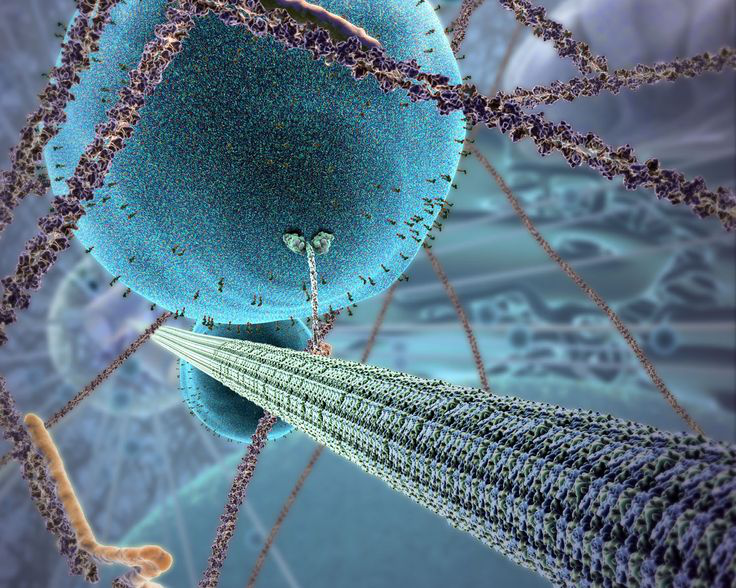
\includegraphics[width=0.7\textwidth]{kinesin_graphic.png}
  \caption{Kinesin-1 with cargo on microtubules	\cite{kinesin_graphic}}
  %\label{fig:https://de.pinterest.com/pin/565905509397043812/}
\end{figure}
\end{titlepage}

\tableofcontents
\pagebreak

%------------------------
\section{Basics}

Proteins are the basis of every living organism. They perform all types of work inside the cells. In this experiment, the interaction of the cytoskeletal motor protein kinesin-1 with microtubule filaments is investigated at two different temperatures.

\subsection{Microtubules}

Microtubules are hollow polymer-cylinders. They are highly dynamic filaments, always shrinking or growing, which serve as tracks for active intercellular transport. Microtubules consists of tubulin subunits, which give the tubules a plus and minus end, which allow a directed transport. 
In this experiment, the dynamic of the tubules is stopped by Taxol. The microtubules are labelled with rhodamine to allow red fluorescence.

\subsection{Kinesin-1}

Kinesin-1 is a motor protein which transports cargo around the cell. It consists of two identical, connected subunits which both have a head, a stalk and a tail. The head serves as motor, the tail as cargoholder. 
The movement of kinesin-1 is accomplished through bipedal walk along microtubules: one head moves in front, the other stays connected to the microtubule. For each step, the kinesin-1 “consumes” one ATP-molecule to reach the needed energy. In this way the protein manages to accomplish a velocity of 0.8$\mu m/s$. However, with a probability of 1\% both heads disconnect, resulting in a detachment of the microtubule after an average way length of 0.8$\mu m$.
In this experiment, the kinesin-1 proteins are labelled with GFP to provide green fluorescence.

\subsection{Fluorescence microscopy}

To investigate the proteins fluorescence microscopy is used. The rhodamine and the GFP are excited by light: One of their electrons enters an excited orbital. This electron has the opposite spin of the remaining electron in the ground-state orbital. The molecules begin to vibrate and lose thermic energy in the process. After around 10\textsuperscript{-8} seconds the excited electron jumps back to the ground state and emits a photon. Because of the lost energy, the emitted photon has a larger wavelength then the absorbed one and can be distinguished from the laser light. Through this the tubules and proteins with the excited molecules can be observed. 
To limit the fluorescing volume, Total Internal Reflection Fluorescence Microscopy is used. The exciting laser lights are totally reflected before they enter the object. However, an evanescent wave enters the object. Like this, only the first few microtubules and proteins are illuminated.


\section{Experimental procedure}

The movement of kinesin-1 has to be researched at two different temperatures: $25^\circ\text{C}$ and $37^\circ\text{C}$.
At first one prepares a flow-cell: two pieces of glass – one hydrophob, one hydrophil to provide a better flow of the liquids – are fused with 3 pieces of parafilm to form two channels, one as a backup. Then the channels are flushed with BRB80 – this is done after every flushing, to wash the channels, keep them wet and provide a good environment for the experiment. Then Anti-Tubulin antibodies, to bind the microtubules in the channels, and F127, to prevent the binding of the kinesin-1 with the glass, are put inside. After this the microtubules, are flushed in. After a waiting time of around 1h the kinesin-1 final solution, which includes the kinesin-1, nutrients for both the microtubules and the kinesin-1 and ATP for the movement of the kinesin-1, is flushed in.
To see the behaviour the samples are researched with a TIRF-microscope with a magnification of 100x and a camera pixel-size of 16$\mu m\textsuperscript{2}$. At first a photo of the microtubules is taken at normal light, to determine the position of the microtubules. After this a 1000-frames video is taken under green laser light, to see the movement of the kinesin-1. The data-analysis is done using the FIESTA-program which is contributed. Here the lines of the microtubules are marked and, after the computer marked tracks of moving particles on this lines, for each temperature 200-500 recognizable tracks are marked. The program calculates the velocity and run-length of this marked tracks.

\section{Experimental data}

\section{Analysis}

\section{Conclusion}

%------------------------

\begin{thebibliography}{9}

\bibitem{kinesin_graphic}
  https://de.pinterest.com/pin/565905509397043812/

\end{thebibliography}

\end{document}
